

\begin{figure}[ht!]
\centering
\subfloat[][HDR]{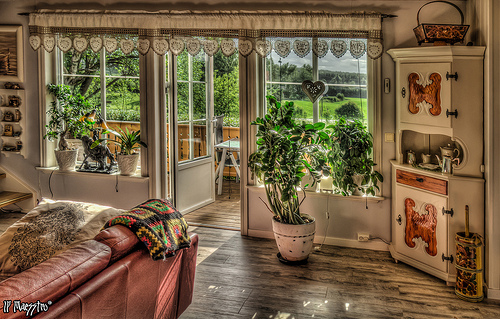
\includegraphics[width=\samplewidth]{../arxiv/figures/flickrDatasetExamples/9566063566_a26f090068.jpg}}~
\subfloat[][Long Exposure]{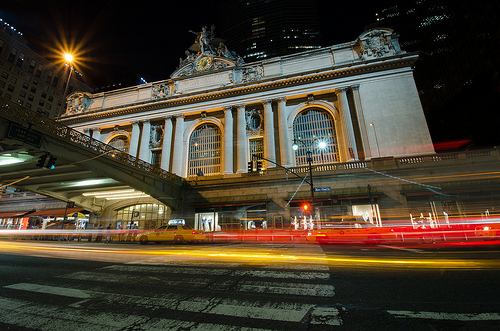
\includegraphics[width=\samplewidth]{../arxiv/figures/flickrDatasetExamples/9558960217_7056981249.jpg}}~
\subfloat[][Macro]{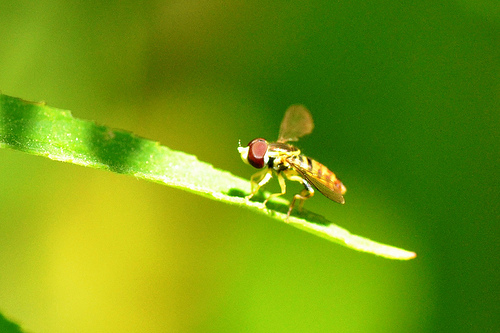
\includegraphics[width=\samplewidth]{../arxiv/figures/flickrDatasetExamples/9550304852_99568eec75.jpg}}
\vspace{-2ex}

\subfloat[][Vintage]{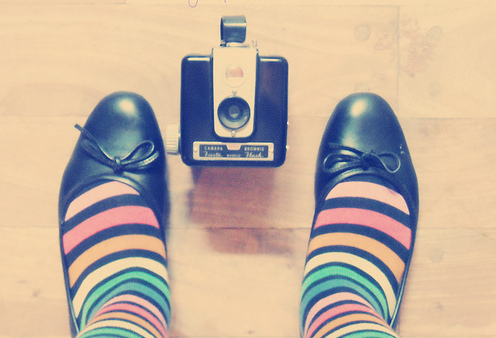
\includegraphics[width=\samplewidth]{../arxiv/figures/flickrDatasetExamples/5863276871_8bf39b0177_crop.jpg}}~
\subfloat[][Romantic]{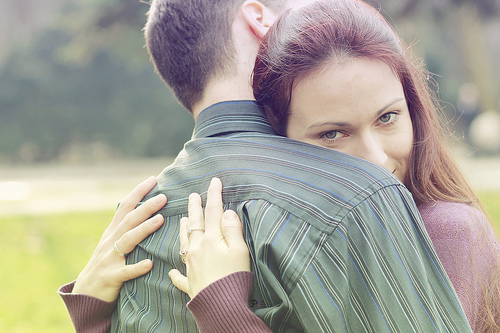
\includegraphics[width=\samplewidth]{../arxiv/figures/flickrDatasetExamples/8546146794_a60b92a504.jpg}}~
\subfloat[][Horror]{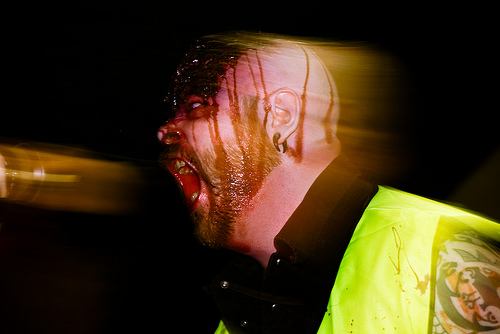
\includegraphics[width=\samplewidth]{../arxiv/figures/flickrDatasetExamples/3444380200_0941a7ce5b.jpg}}
\vspace{-2ex}

\subfloat[][Minimal]{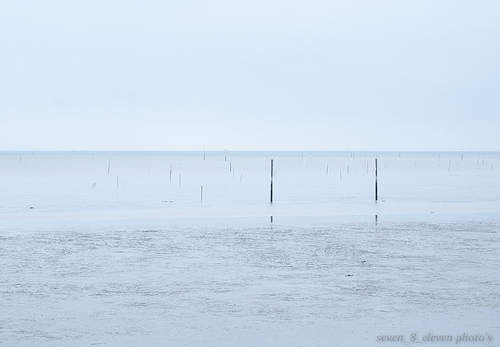
\includegraphics[width=\samplewidth]{../arxiv/figures/flickrDatasetExamples/9039257065_8a87e1f3f6.jpg}}~
\subfloat[][Hazy]{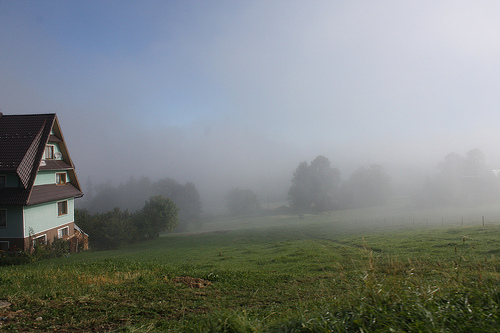
\includegraphics[width=\samplewidth]{../arxiv/figures/flickrDatasetExamples/6588242067_c0a74e7da0.jpg}}~
\subfloat[][Noir]{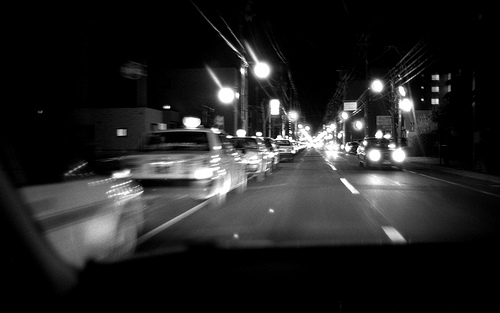
\includegraphics[width=\samplewidth]{../arxiv/figures/flickrDatasetExamples/3427272477_444a9a038d.jpg}}
%\vspace{-2ex}

\caption{
    Typical images in different style categories of our Flickr Style dataset.
    The dataset comprises 18 styles in total, each with 3,000 examples.
}
\label{fig:flickr_style_examples}
\end{figure}
\section{Introduction}

Images convey meaning in multiple ways; \textit{visual style} is often a significant component of image meaning for creative images.
For example, the same scene portrayed in
the lush, springtime colors of a Renoir painting would tell a different story than shown in the harsh, dark tones of a typical horror movie.
Visual style is crucial to how a viewer interprets an image in many contexts, including art, design, entertainment, advertising, and social media.
%It plays a major role in creative tasks such as illustrating articles, presentations, creating and editing photographs, and other design work.
Moreover, an increasing amount of visual media consumption though online social media feeds, photo sharing sites, and news sites,
is now curated by machines and not people.
%Indeed, automatic approaches (such as Google+ Photos) now edit and even create visual content from source materials.
Yet, virtually no research in computer vision has explored visual style.

This paper introduces new approaches and datasets for the automatic analysis of image style.
Visual style is very recognizable to human viewers, yet difficult to define precisely. Style may combine aspects of color, lighting, composition, scene objects, and other facets. Hence, we prefer to define style empirically through labelled data, and then analyze the divisions between these classes.
Finding existing datasets insufficient, %\holger{I assume we expand this in the related work section. I.e. which datasets we are referring to and why they are insufficient},
we gather a new large-scale dataset of photographs annotated with diverse visual style labels.
This dataset embodies several different aspects of visual style, including photographic techniques (``Macro," ``HDR"), composition styles (``Minimal," ``Geometric"),
moods (``Serene," ``Melancholy"), genres (``Vintage," ``Romantic," ``Horror"),
and types of scenes (``Hazy,'' ``Sunny''). %\holger{I do remember an early discussion on style classification versus scene classification. Is it really different? I imagine the machinery to distinguish a beach image from a cityscape, from a forest picture, from a portrait is quite similar to our style detection machinery. If so, what is different? Are we discussing this in the related work section?}
We  also gather a large dataset of visual art (mostly paintings) annotated with art historical style labels, ranging from Renaissance to modern art.
We perform a thorough evaluation of different visual features for the task of predicting these style annotations.
We find that ``deep'' features trained on a large amount of data labeled with object class categories (ImageNet) perform significantly better than traditionally used hand-designed features.

The style predictors that our datasets and learning enable are useful as mid-level features in their own right.
When making presentations, a searchable source of stylistically coherent images would be useful.
A story may be illustrated with images that match not only its objective content, but also its sentiment.
In addition to evaluating classification performance of our approach, we demonstrate an application of style classifiers to visual search, making a large image collection searchable by both content tags and visual style (``bird, bright/energetic," ``train, film noir").
Additionally, we demonstrate that styles learned from paintings can be used to search collections of photographs, and vice versa.

%Additionally, we enable visual similarity search results to be filtered by visual style, making possible queries such as ``similar to this image, but scarier''.

All data, trained predictors, code, and a web-based user interface for searching image collections ``with style'' will be released upon publication.

\begin{figure} %[ht]
\centering

\subfloat[][Baroque]{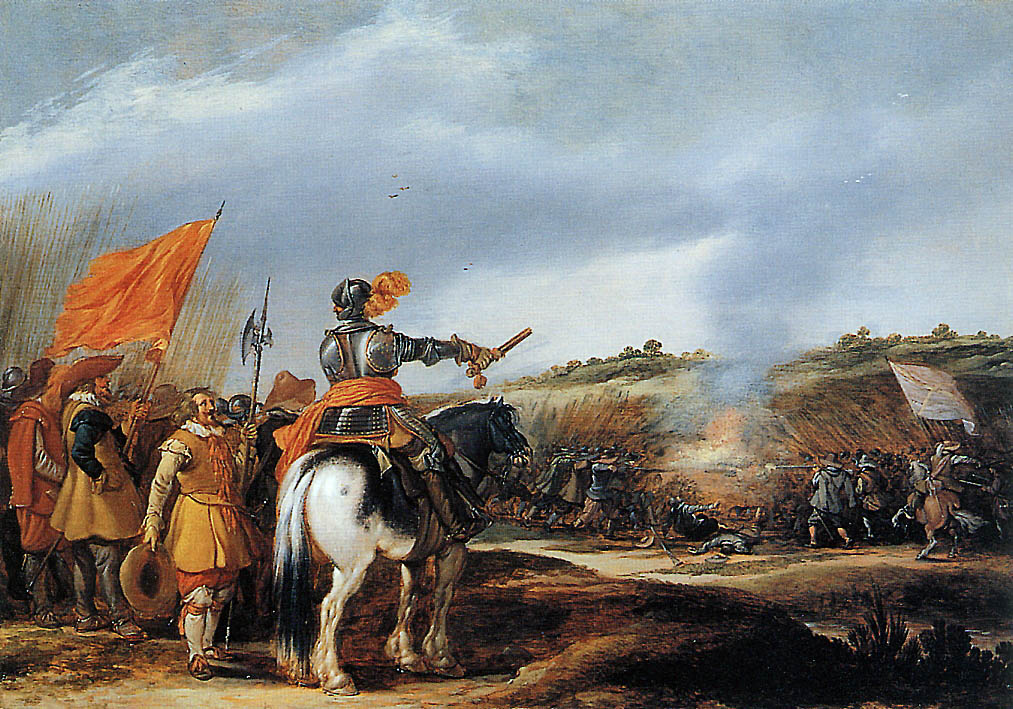
\includegraphics[width=\samplewidth]{../arxiv/figures/wikipaintingsDatasetExamples/adriaen-van-de-velde-battle.jpg}}~
\subfloat[][Rococo]{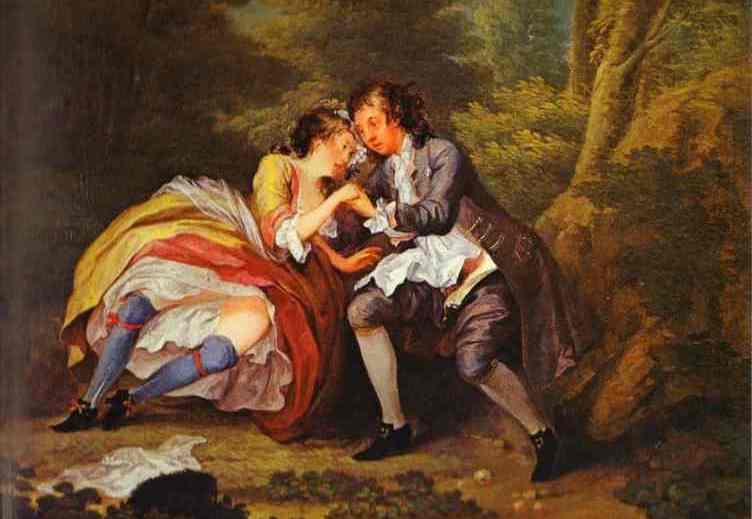
\includegraphics[width=\samplewidth]{../arxiv/figures/wikipaintingsDatasetExamples/william-hogarth-after-outdoor-scene-crop.jpg}}~
\subfloat[][Northern Renaissance]{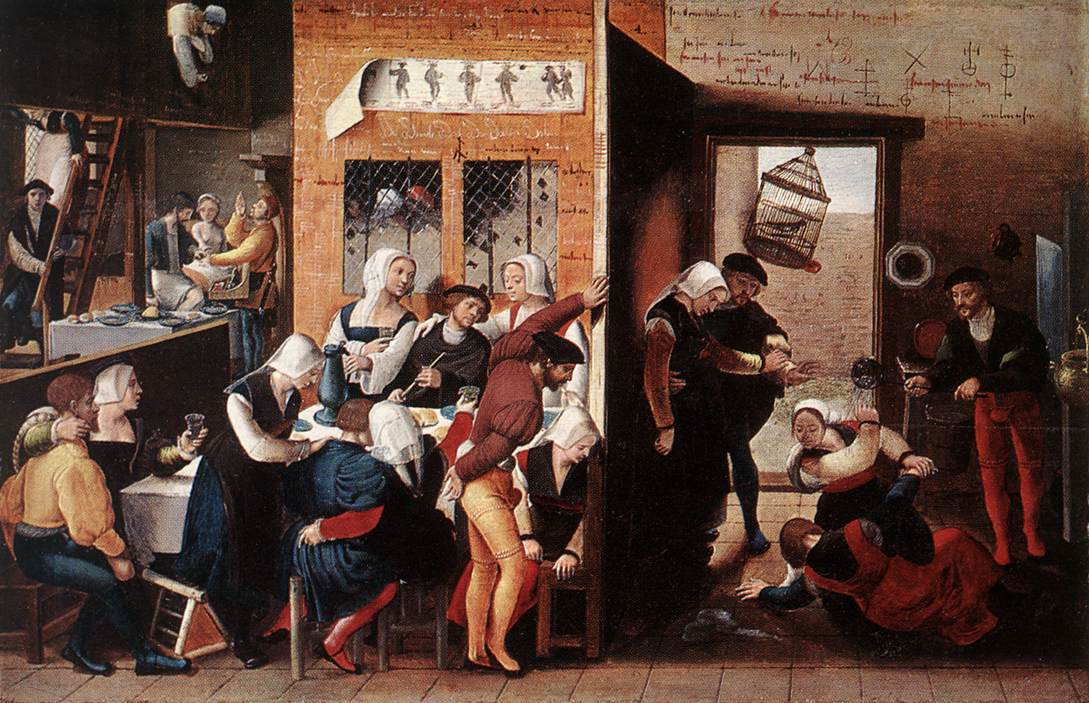
\includegraphics[width=\samplewidth]{../arxiv/figures/wikipaintingsDatasetExamples/jan-van-hemessan-a-merry-company.jpg}}
\vspace{-2ex}

\subfloat[][Impressionism]{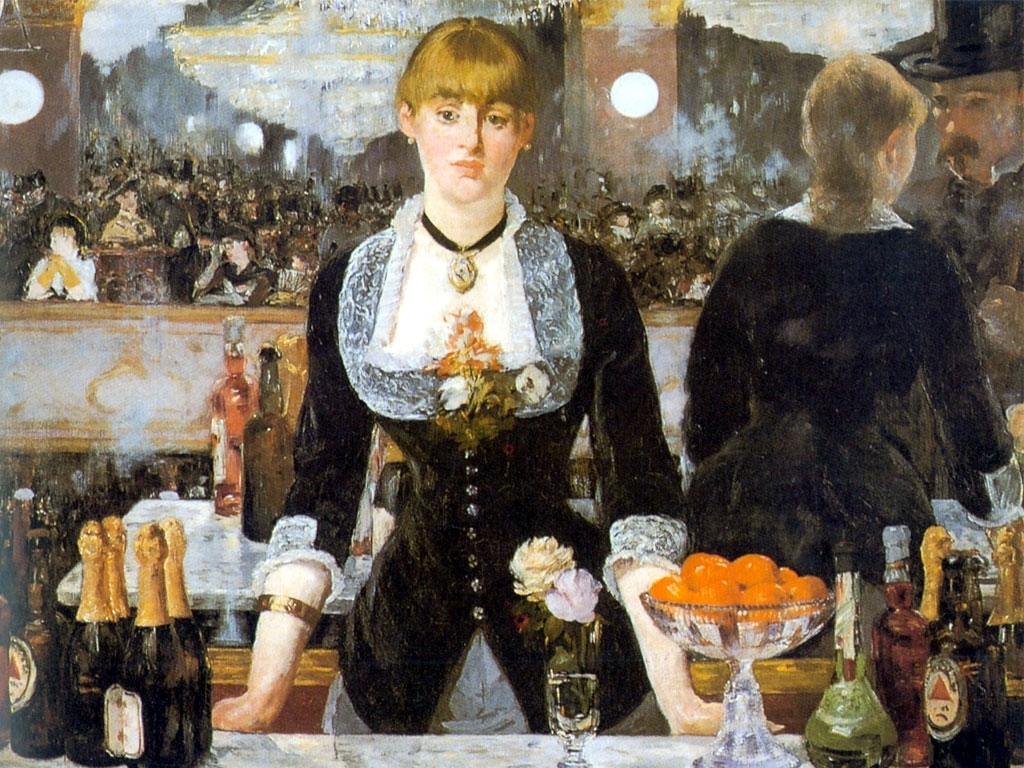
\includegraphics[width=\samplewidth]{../arxiv/figures/wikipaintingsDatasetExamples/a-bar-at-the-folies-bergere-1882-1.jpg}}~
\subfloat[][Post-Impressionism]{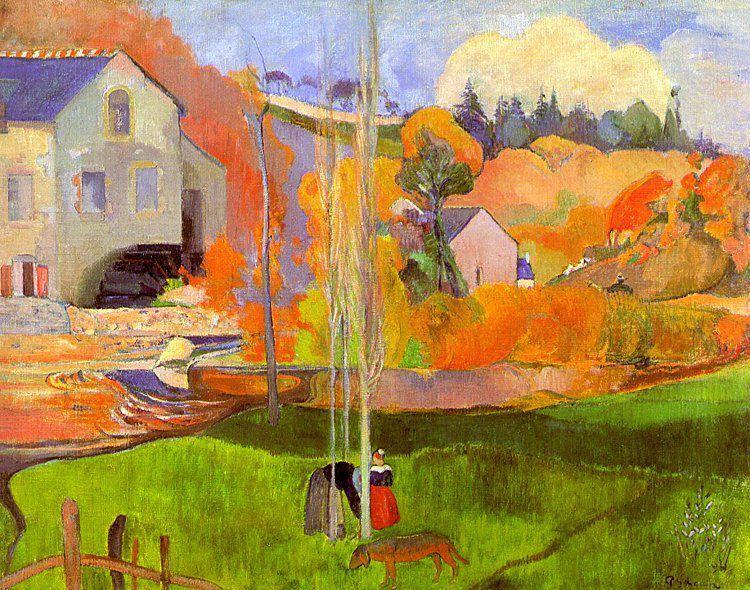
\includegraphics[width=\samplewidth]{../arxiv/figures/wikipaintingsDatasetExamples/a-breton-landscape-david-s-mill-1894.jpg}}~
%\subfloat[][Surrealism]{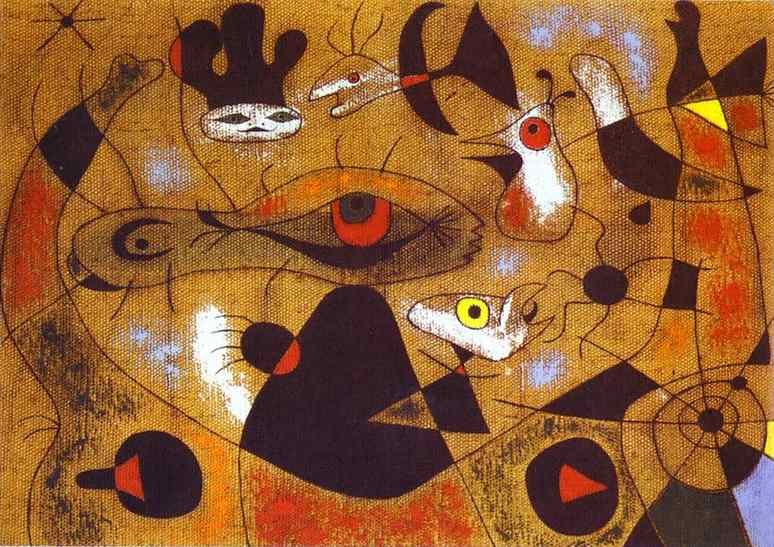
\includegraphics[width=\samplewidth]{a-dew-drop-falling-from-a-bird-s-wing-wakes-rosalie-who-has-been-asleep-in-the-shadow-of-a.jpg}
\subfloat[][Ukiyo-e]{
\includegraphics[width=\samplewidth]{../arxiv/figures/wikipaintingsDatasetExamples/asakusa-honganji-temple-in-th-eastern-capital.jpg}}
%\subfloat[][Cubism]{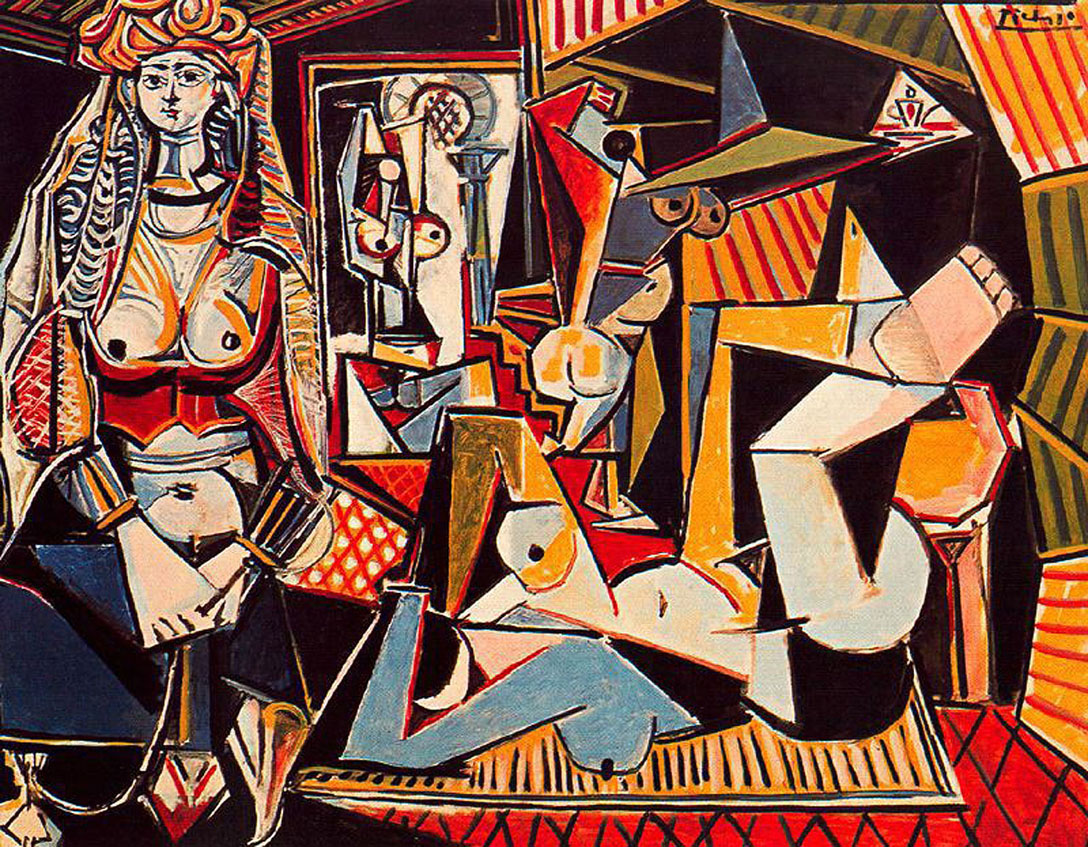
\includegraphics[width=\samplewidth]{picasso-algerian-women-delacroix-1955.jpg}
\vspace{-2ex}

\subfloat[][Abs.~Expressionism]{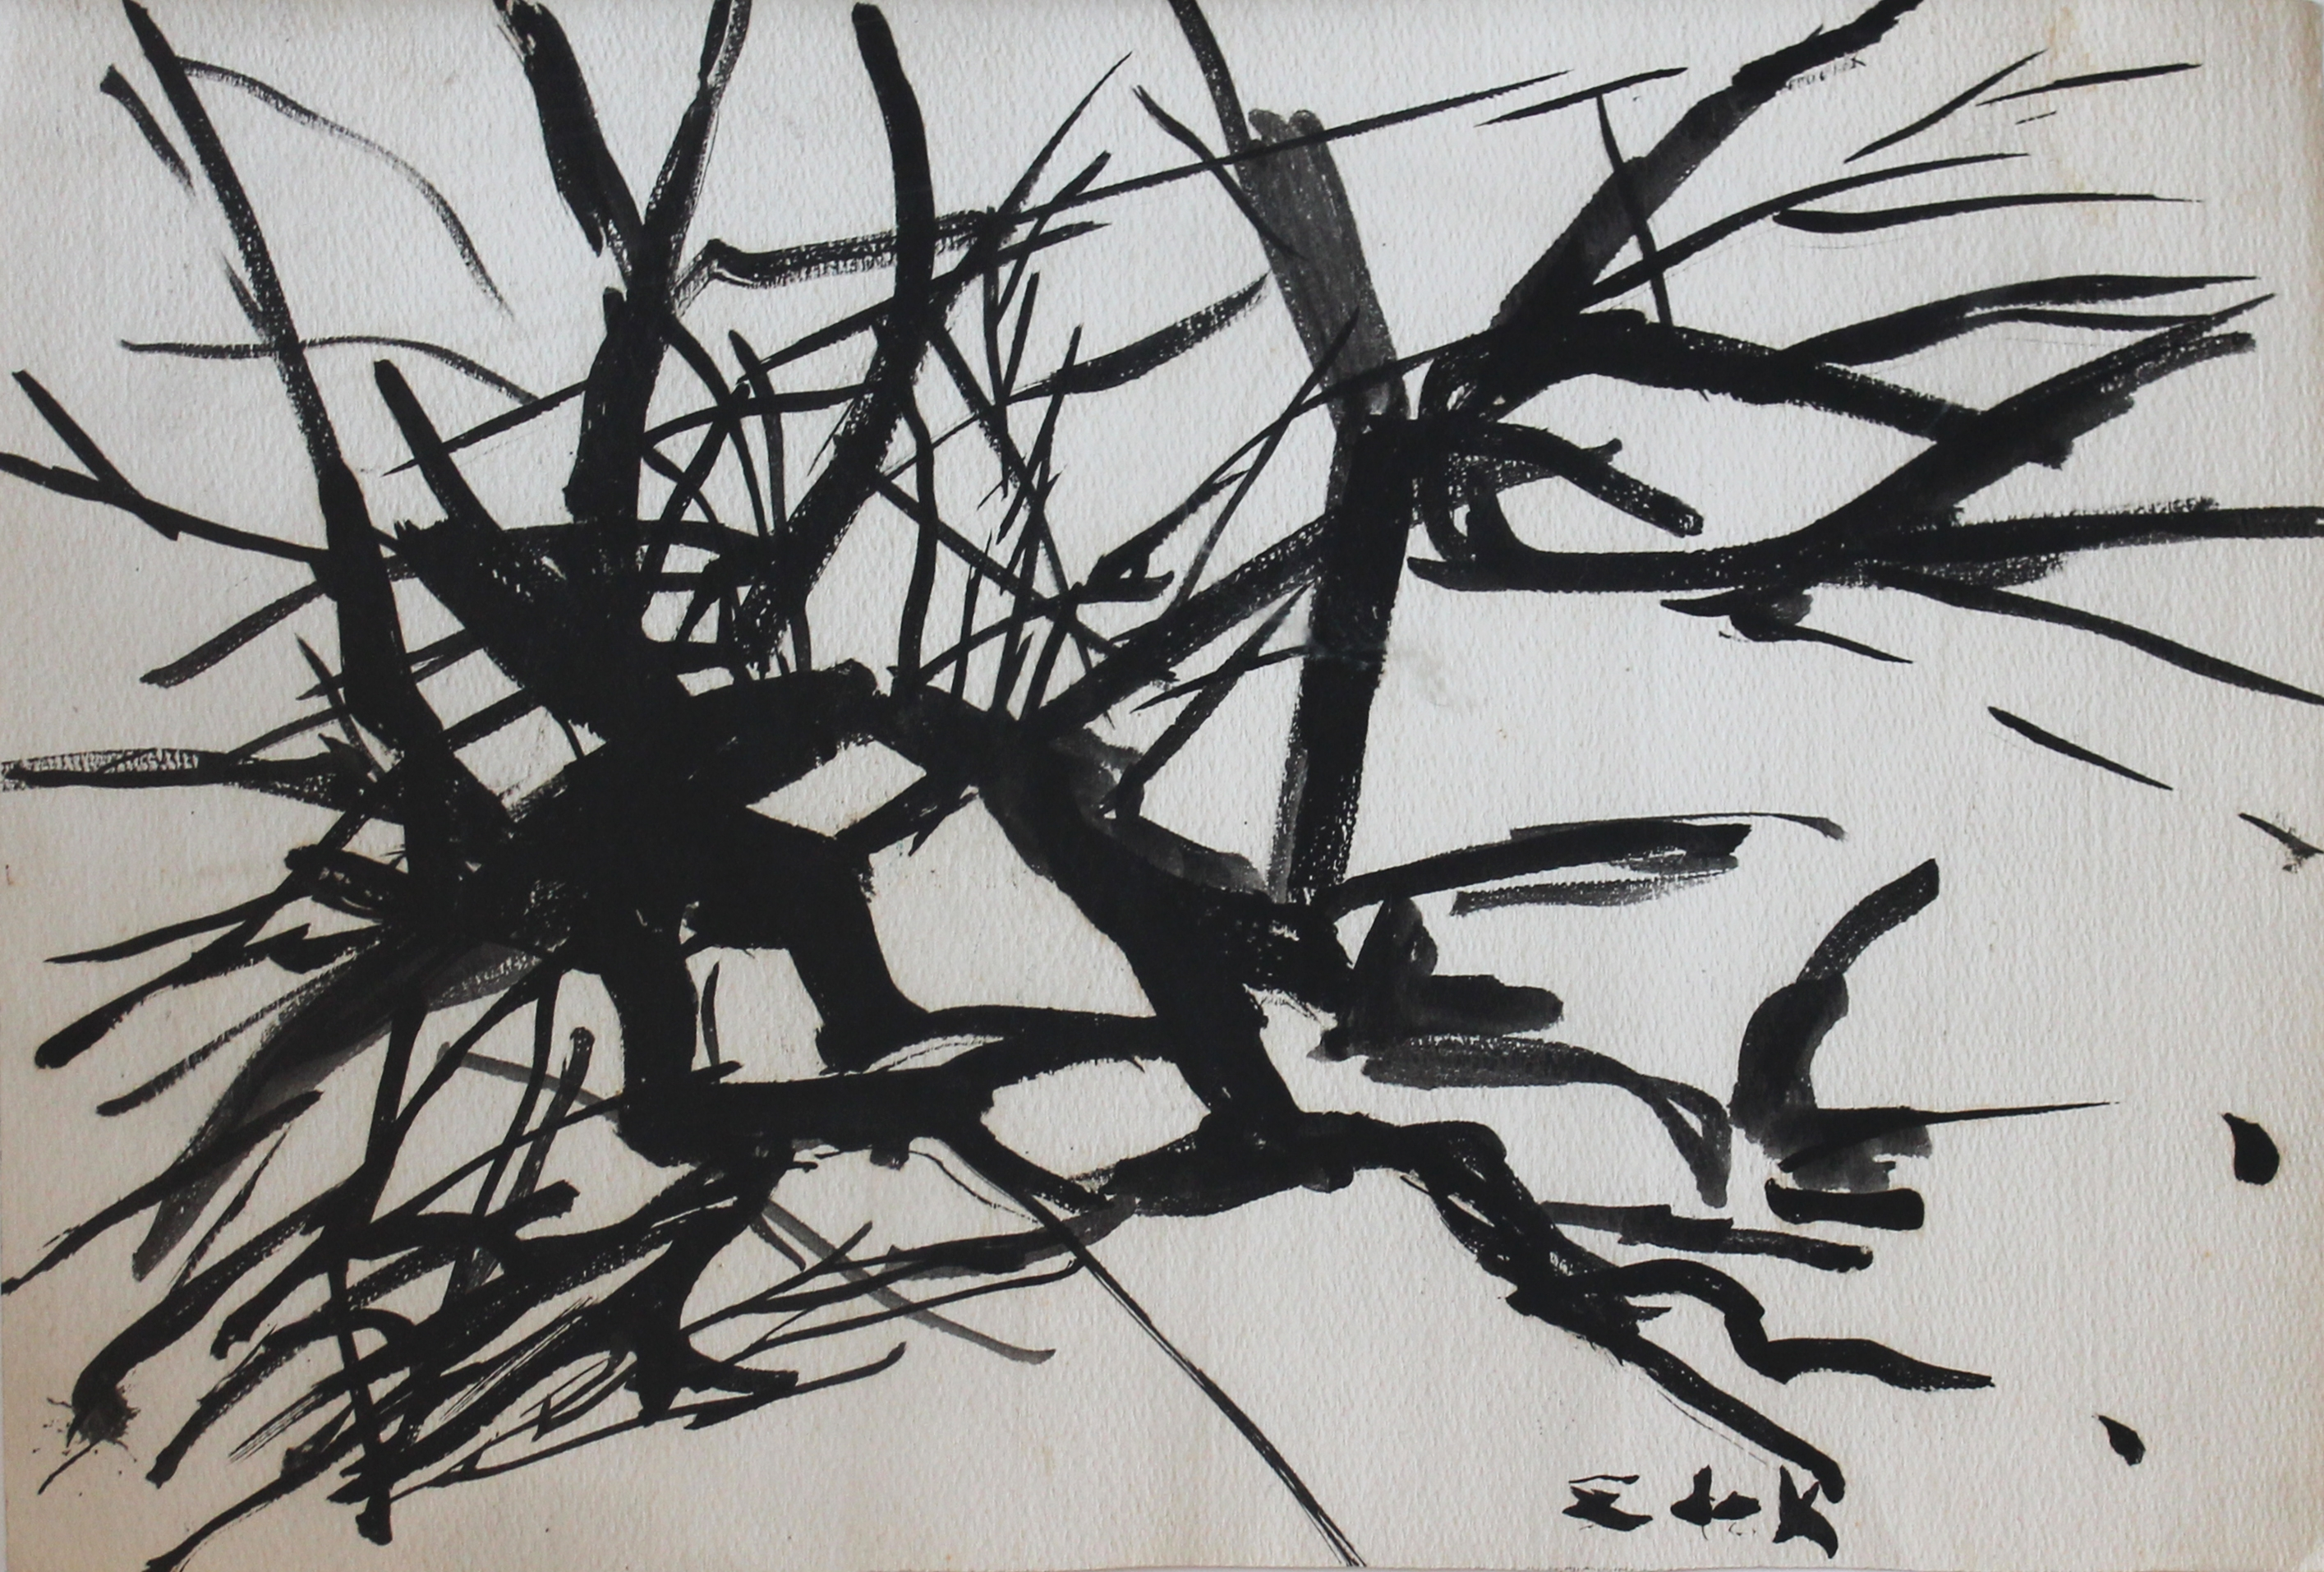
\includegraphics[width=\samplewidth]{../arxiv/figures/wikipaintingsDatasetExamples/elaine-de-kooning-abstract-1970.jpg}}~
\subfloat[][Minimalism]{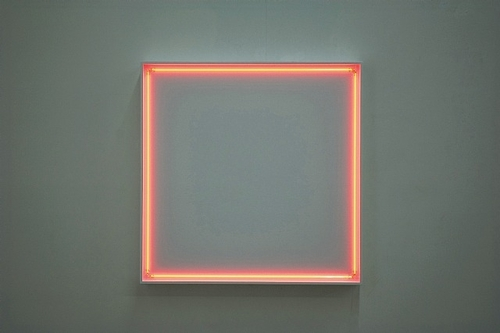
\includegraphics[width=\samplewidth]{../arxiv/figures/wikipaintingsDatasetExamples/4-rythmes-interf-rents-en-formant-un-carr-1972.jpg}}~
\subfloat[][Color Field Painting]{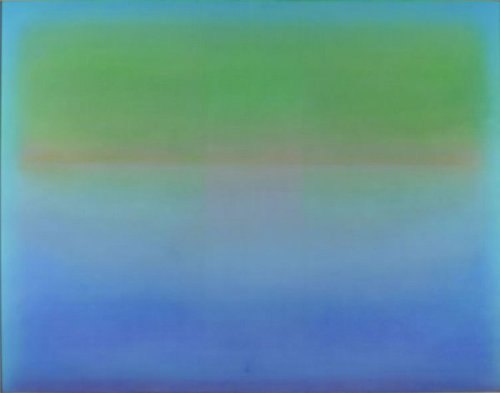
\includegraphics[width=\samplewidth]{../arxiv/figures/wikipaintingsDatasetExamples/leon-berkowitz-after-the-cloud.jpg}}
\vspace{-2ex}

\caption{
    Typical images in different style categories from our Wikipaintings dataset.
    The dataset comprises 85,000 images labeled with 22 art historical styles.
}
\label{fig:wikipaintings_examples}
\end{figure}
